\documentclass{article}
\usepackage{iclr2024_conference,times}

\input{math_commands.tex}

\usepackage{hyperref}
\usepackage{url}
\usepackage{booktabs}
\usepackage{graphicx}
\usepackage{multirow}
\usepackage{amsmath}

\title{Denoising Autoencoders for Parkinson's Disease\\Wrist IMU Signals}

\author{Wanghley Soares Martins \And Yibei Gou \\
Department of Electrical and Computer Engineering \\
Duke University \\
\texttt{\{wanghley.martins, yibei.gou\}@duke.edu}
}

\newcommand{\fix}{\marginpar{FIX}}
\newcommand{\new}{\marginpar{NEW}}

\iclrfinalcopy
\begin{document}

\maketitle

% ──────────────────────────────────────────────────────────────────
\begin{abstract}
We design and evaluate denoising autoencoders (DAEs) for 6-channel inertial
measurement unit (IMU) signals from the PADS Parkinson's Disease Smartwatch
dataset \citep{varghese2023pads,physionet2000}.
Five encoder-decoder architectures are compared—Fully-Connected (FC),
1D-CNN, LSTM, UNet-1D, and a patch-based Transformer—under four noise
regimes: Gaussian, random masking, impulse, and sinusoidal interference.
Models are trained to reconstruct clean signals from artificially corrupted
inputs using a hybrid time-frequency loss.
We conduct systematic experiments on architecture comparison, latent-dimension
sensitivity, noise-level robustness, noise-type cross-evaluation, and
hyperparameter tuning.
Reconstruction quality is measured by MSE, SNR improvement (SNRi), and a
domain-specific tremor-band power metric targeting the clinically relevant
4--6\,Hz range in Parkinson's Disease.
Skip-connection and attention-based architectures substantially outperform
purely sequential models, and the spectral loss term preserves
frequency content beyond what MSE alone encourages.
\end{abstract}

% ──────────────────────────────────────────────────────────────────
\section{Introduction}
\label{sec:intro}

Parkinson's Disease (PD) is the second most prevalent neurodegenerative
disorder worldwide, affecting over 10 million people \citep{poewe2017parkinson}.
Its cardinal motor symptom—resting tremor at 4--6\,Hz—is directly observable
in wrist accelerometry and gyroscopy signals from commodity smartwatches,
making wearable sensing an attractive non-invasive monitoring modality.
However, raw IMU recordings are corrupted by motion artifacts, sensor dropout,
ambient vibrations, and electrode noise that degrade downstream analysis.

Denoising autoencoders \citep{vincent2008extracting,vincent2010stacked} offer a
principled framework for signal recovery: a neural network $f_{\vtheta}$ is
trained to map a corrupted observation $\vx_{\text{noisy}}$ back to the clean
signal $\vx$, learning a structured latent representation along the way:
%
\begin{equation}
  \hat{\vx} = f_{\vtheta}(\vx_{\text{noisy}}),
  \qquad
  \mathcal{L}(\vtheta) = \E\bigl[\|\vx - f_{\vtheta}(\vx_{\text{noisy}})\|_2^2\bigr].
  \label{eq:dae}
\end{equation}
%
Beyond practical denoising, the bottleneck latent vector $\vz$ encodes a
compressed representation of the temporal dynamics that could be used for
downstream tasks such as tremor severity scoring or gait analysis.

This project contributes:
(1) a complete denoising pipeline for 6-channel smartwatch IMU data using
    subject-level train/val/test splits that prevent patient-level leakage;
(2) implementation and comparison of five autoencoder architectures spanning
    the FC, CNN, LSTM, skip-connection (UNet), and Transformer families;
(3) four noise models covering additive, masking, impulsive, and interference
    corruption;
(4) five systematic experiments including architecture comparison, latent-dimension
    ablation, noise robustness, noise-type cross-evaluation, and
    hyperparameter search; and
(5) a clinically motivated tremor-band power MAE metric for the 4--6\,Hz range.

% ──────────────────────────────────────────────────────────────────
\section{Dataset}
\label{sec:dataset}

\subsection{PADS — Parkinson's Disease Smartwatch Dataset}

We use the PADS dataset \citep{varghese2023pads}, publicly available on
PhysioNet \citep{physionet2000}.
It contains wrist IMU recordings from 469 subjects collected with Apple Watch
Series 4 at 100\,Hz across six diagnostic groups.
We restrict our study to \textbf{Parkinson's Disease (276 subjects)} and
\textbf{Healthy Controls (79 subjects)}, totalling 355 subjects,
to maintain a clinically interpretable binary contrast.

Each subject performed \textbf{11 standardised motor tasks}:
\textit{Relaxed}, \textit{RelaxedTask}, \textit{CrossArms}, \textit{StretchHold},
\textit{HoldWeight}, \textit{LiftHold}, \textit{PointFinger},
\textit{TouchIndex}, \textit{TouchNose}, \textit{DrinkGlas}, and
\textit{Entrainment} (rhythmic cueing).
Raw recordings are stored as comma-separated files with 7 columns
(Time, Accel$_{X/Y/Z}$, Gyro$_{X/Y/Z}$);
we discard the timestamp and retain all \textbf{6 sensor channels}.

\subsection{Preprocessing}

\textbf{Vibration artifact removal.}
The first 50 samples of every recording contain a smartwatch vibration artifact
from the task-start notification and are discarded before windowing.

\textbf{Fixed-length windowing.}
Recordings are segmented into non-overlapping windows of
$L = 1024$ samples (10.24\,s).
During training, overlapping windows with hop size 128 are also generated
(87.5\% overlap), yielding $\approx 8\times$ more training examples per recording
as data augmentation; evaluation uses non-overlapping windows only.

\textbf{Robust CSV parsing.}
Some files contain malformed rows from recording interruptions.
We use \texttt{pandas.read\_csv} with \texttt{on\_bad\_lines='skip'}
and subsequently remove rows containing NaN values.

\textbf{Z-score normalisation.}
Per-channel mean $\mu_c$ and standard deviation $\sigma_c$ are computed over
all training-set windows and applied consistently to validation and test splits:
$\tilde{x}_c = (x_c - \mu_c) / (\sigma_c + \epsilon)$, $\epsilon = 10^{-8}$.

\subsection{Subject-Level Data Split}
\label{sec:split}

To prevent patient-level data leakage, the split is performed
\textbf{by subject}, not by window.
Subject IDs are shuffled with a fixed seed and divided 80/10/10:
$\approx$197 training subjects ($\approx$10\,300 windows with augmentation),
$\approx$25 validation subjects ($\approx$520 windows), and
$\approx$25 test subjects ($\approx$520 windows).
Only subjects with at least one downloaded timeseries file are included.

% ──────────────────────────────────────────────────────────────────
\section{Noise Models}
\label{sec:noise}

All four corruption functions operate on tensors of shape
$(B, C, L)$ and are applied independently at each training step,
so the model never sees the same corrupted version twice.

\textbf{Gaussian noise.} $\vx_{\text{noisy}} = \vx + \boldsymbol{\varepsilon}$,
$\boldsymbol{\varepsilon} \sim \mathcal{N}(\mathbf{0}, \sigma^2 \mathbf{I})$.
Default $\sigma = 0.1$; swept over $\{0.05, 0.1, 0.2, 0.4\}$.

\textbf{Random masking.}
Contiguous segments are zeroed out with mask-start probability $p = 0.1$
and segment length 20 samples (200\,ms).
The \emph{same} time mask is applied across all channels, simulating a
physical sensor dropout rather than per-channel noise.

\textbf{Impulse noise.}
Random large-amplitude spikes are inserted:
$x_{\text{noisy}}[t] = x[t] + A \cdot s[t] \cdot \mathbf{1}[u[t] < p_{\text{imp}}]$
with $A = 3.0$, $p_{\text{imp}} = 0.05$, and $s[t] \in \{-1, +1\}$.

\textbf{Sinusoidal interference.}
A fixed-frequency tone is added:
$\vx_{\text{noisy}} = \vx + A\sin(2\pi f L \cdot t)$, $t \in [0,1]$,
with $A = 0.3$ and $f = 0.05$, broadcasting across all channels.

% ──────────────────────────────────────────────────────────────────
\section{Model Architectures}
\label{sec:models}

All five architectures follow the encoder-decoder structure of
Eq.~\eqref{eq:dae} with a $d_z$-dimensional bottleneck (default $d_z = 64$).
Input and output tensors have shape $(B, 6, 1024)$.

\subsection{Fully-Connected Autoencoder (FC)}

The FC autoencoder serves as the lower-bound baseline with no inductive bias.
The input window is flattened to $\mathbb{R}^{6144}$ before encoding:
%
\begin{equation*}
  \underbrace{6{\times}1024}_{\text{flatten}} \to 256 \to 128 \to d_z
  \quad \xrightarrow{\text{decoder}} \quad
  d_z \to 128 \to 256 \to 6{\times}1024.
\end{equation*}
%
Each hidden layer uses ReLU activations and Dropout ($p = 0.2$) to mitigate
overfitting. \textbf{Parameters:} 3.23M.

\subsection{1D Convolutional Autoencoder (CNN)}

The CNN exploits local temporal patterns through strided convolutions that
progressively compress the time dimension:
$L \to L/2 \to L/4 \to L/8 \to L/16$, with channels $6 \to 32 \to 64 \to 128 \to 256$.
Each encoder layer applies Conv1d (kernel~3, stride~2, padding~1), ReLU, and
Dropout ($p = 0.1$).
The bottleneck flattens the $(256, 64)$ feature map and projects to $d_z$ via
a linear layer.
The decoder mirrors this with ConvTranspose1d (kernel~4, stride~2)
to upsample back to the original length.
\textbf{Parameters:} 2.42M.

\subsection{LSTM Autoencoder}

The LSTM models long-range temporal dependencies through gated recurrent units.

\textbf{Encoder.}
The signal is transposed to $(B, L, C)$ and fed to a 2-layer bidirectional
LSTM (hidden size 128).
Rather than mean-pooling over all 1024 time steps (which causes vanishing
gradients), we concatenate the \emph{final} forward and backward hidden states
of the top layer to form a $(B, 256)$ context vector, then project linearly to
$d_z$.

\textbf{Decoder.}
Two separate linear projections map $\vz$ to the initial hidden
state $\mathbf{h}_0$ and cell state $\mathbf{c}_0$ of a 2-layer unidirectional
LSTM (hidden size 128).
Zero-valued inputs of shape $(B, L, C)$ are fed as the input sequence,
allowing the LSTM to generate the reconstruction entirely from its initialised
state.
An output linear layer projects each time step to $C$ channels.
Dropout ($p = 0.2$) is applied between LSTM layers.
\textbf{Parameters:} 787K.

\subsection{1D UNet Autoencoder (UNet-1D)}

The UNet architecture \citep{ronneberger2015unet} augments the CNN
encoder-decoder with \textbf{skip connections} that concatenate encoder feature
maps directly into the corresponding decoder stage.
This allows the decoder to access fine-grained local structure without routing
it through the bottleneck—particularly beneficial for preserving high-frequency
tremor bursts.
Four encoder blocks (Conv1d, stride~2) feed a linear FC bottleneck; four decoder
blocks (ConvTranspose1d, stride~2) receive the corresponding encoder outputs
concatenated along the channel axis before each convolution.
\textbf{Parameters:} 2.46M.

\subsection{Patch-Based Transformer Autoencoder}

Applying full self-attention to $L = 1024$ time steps incurs
$\mathcal{O}(L^2) = \mathcal{O}(10^6)$ cost per head per layer.
We address this with a ViT-style patching strategy
\citep{dosovitskiy2021vit}: the signal is divided into 128 non-overlapping
patches of 8 samples each, reducing attention complexity to
$\mathcal{O}(128^2)$---64$\times$ smaller---while preserving all temporal content.

Each patch $\in \mathbb{R}^{6 \times 8}$ is linearly projected to
$d_{\text{model}} = 128$.
Learnable positional embeddings of shape $(1, 128, 128)$ are added.
Two Pre-LN Transformer encoder layers
($n_{\text{heads}} = 4$, $d_{\text{ff}} = 256$, dropout~0.1) \citep{vaswani2017attention}
encode the tokens; mean pooling over the patch dimension followed by a linear
projection gives the latent $\vz$.
The decoder tiles $\vz$ back to $(B, 128, d_{\text{model}})$, adds
positional embeddings, refines with two further Transformer encoder layers,
and reconstructs each patch via a linear layer.
\textbf{Parameters:} 575K.

\subsection{Architecture Summary}

\begin{table}[h]
\caption{Architecture properties. All models share $d_z = 64$, $C = 6$, $L = 1024$.}
\label{tab:arch-summary}
\begin{center}
\begin{tabular}{lrllc}
\toprule
\textbf{Architecture} & \textbf{Params} & \textbf{Temporal bias} & \textbf{Range} & \textbf{Skip} \\
\midrule
FC           & 3.23M  & None (global)       & Global  & No  \\
CNN          & 2.42M  & Local patterns      & Local   & No  \\
LSTM         & 787K   & Sequential/recurrent& Long    & No  \\
UNet-1D      & 2.46M  & Local patterns      & Local   & Yes \\
Transformer  & 575K   & Self-attention      & Global  & No  \\
\bottomrule
\end{tabular}
\end{center}
\end{table}

% ──────────────────────────────────────────────────────────────────
\section{Training Procedure}
\label{sec:training}

\subsection{Hybrid Loss Function}

We use a hybrid reconstruction loss combining time-domain MSE with a
frequency-domain spectral term:
%
\begin{equation}
  \mathcal{L}(\vtheta)
  = \underbrace{\|\hat{\vx} - \vx\|_2^2}_{\text{MSE}}
  + \;\alpha\;\underbrace{\bigl\||\mathcal{F}(\hat{\vx})| - |\mathcal{F}(\vx)|\bigr\|_1}_{\text{spectral } L_1}
  \label{eq:loss}
\end{equation}
%
with $\alpha = 0.1$.
The FFT is computed along the time axis with orthonormal normalisation.
The spectral term encourages preservation of frequency content—particularly
the 4--6\,Hz tremor band—even when time-domain alignment is imperfect.

\subsection{Optimisation}

All models are trained with Adam \citep{kingma2015adam} (weight decay $10^{-5}$,
default $\text{lr} = 10^{-3}$) for 100 epochs.
A ReduceLROnPlateau scheduler (factor 0.5, patience 10 epochs) halves the
learning rate when validation loss plateaus.
Gradient clipping (max norm 1.0) stabilises LSTM training.
The model checkpoint with the lowest validation hybrid loss is retained.

Each run is stored under a timestamped directory
(\texttt{results/YYYYMMDD\_HHMMSS/}) alongside a \texttt{run\_config.json}
snapshot of all hyperparameters for full reproducibility.

% ──────────────────────────────────────────────────────────────────
\section{Evaluation Metrics}
\label{sec:metrics}

\textbf{MSE.}
$\text{MSE} = \frac{1}{N}\sum_i \|\hat{\vx}_i - \vx_i\|_2^2$.
Note: the training objective (Eq.~\ref{eq:loss}) includes a spectral term,
so training loss and test MSE are on different scales and should not be compared
directly.
All cross-architecture comparisons use test MSE only.

\textbf{SNR and SNRi.}
$\text{SNR}(\vx, \hat{\vx}) = 10\log_{10}(\|\vx\|_2^2 / \|\vx - \hat{\vx}\|_2^2)$\,[dB].
SNR improvement $\text{SNRi} = \text{SNR}(\vx, \hat{\vx}) - \text{SNR}(\vx, \vx_{\text{noisy}})$
measures the net benefit of denoising over the raw noisy baseline; positive
values indicate successful denoising.

\textbf{Tremor-Band Power MAE.}
A domain-specific metric for Parkinson's:
%
\begin{equation}
  \text{TremorMAE} = \frac{1}{N}\sum_i \bigl| P_{4\text{-}6}(\hat{\vx}_i) - P_{4\text{-}6}(\vx_i) \bigr|,
  \quad P_{4\text{-}6}(\vx) = \!\!\sum_{f \in [4,6]\,\text{Hz}}\!\! |\mathcal{F}(\vx)[f]|^2.
\end{equation}
%
Lower TremorMAE indicates better preservation of the clinically relevant tremor
band.
We report both the \emph{input} TremorMAE (noisy vs.\ clean) and
\emph{output} TremorMAE (reconstruction vs.\ clean).

% ──────────────────────────────────────────────────────────────────
\section{Experiments and Results}
\label{sec:experiments}

\subsection{Experiment 1: Hyperparameter Search}
\label{sec:exp-hyperparam}

A grid search over learning rate $\times$ batch size was performed using the CNN
architecture for 50 epochs.
Table~\ref{tab:hyperparam} reports the best validation hybrid loss for each
combination.

\begin{table}[h]
\caption{Hyperparameter grid search results (CNN, 50 epochs).
Best validation hybrid loss across all epochs; best cell in \textbf{bold}.}
\label{tab:hyperparam}
\begin{center}
\begin{tabular}{lccc}
\toprule
\textbf{Learning Rate} & \textbf{Batch 32} & \textbf{Batch 64} & \textbf{Batch 128} \\
\midrule
$1\times10^{-4}$ & 0.6791 & 0.6816 & 0.7056 \\
$5\times10^{-4}$ & 0.6621 & \textbf{0.6621} & 0.6750 \\
$1\times10^{-3}$ & 0.7042 & 0.7212 & 0.6724 \\
\bottomrule
\end{tabular}
\end{center}
\end{table}

The optimal configuration is $\text{lr} = 5 \times 10^{-4}$, batch size~64.
Validation loss varies by only $\approx$0.06 across the entire grid, suggesting
a flat landscape in this region.
The moderate learning rate outperforms both extremes: $10^{-4}$ converges more
slowly while $10^{-3}$ overshoots.
Batch size 32--64 slightly outperforms 128, as smaller-batch gradient noise acts
as mild regularisation given the moderate dataset size.

\subsection{Experiment 2: Architecture Comparison}
\label{sec:exp-arch}

All five architectures are trained for 100 epochs with Gaussian noise
($\sigma = 0.1$) using the best hyperparameters from Experiment~1.
Table~\ref{tab:arch-results} reports test-set metrics from the best validation
checkpoint.
Figure~\ref{fig:reconstructions} shows example clean, noisy, and reconstructed
signals for each architecture.

\begin{table}[h]
\caption{Architecture comparison under Gaussian noise ($\sigma = 0.1$, 100 epochs).
SNRi $> 0$ indicates improvement over the noisy baseline.}
\label{tab:arch-results}
\begin{center}
\begin{tabular}{lcccc}
\toprule
\textbf{Architecture} & \textbf{Test MSE\,$\downarrow$} & \textbf{SNR$_\text{out}$\,(dB)} & \textbf{SNRi\,(dB)\,$\uparrow$} & \textbf{TremorMAE$_\text{out}$\,$\downarrow$} \\
\midrule
FC          & --- & --- & --- & --- \\
CNN         & --- & --- & --- & --- \\
LSTM        & --- & --- & --- & --- \\
UNet-1D     & --- & --- & --- & --- \\
Transformer & --- & --- & --- & --- \\
\bottomrule
\end{tabular}
\end{center}
\end{table}

\textit{Results pending full experimental run; table will be completed with
final values.}
Preliminary observations (epochs 1--80) indicate clear architectural
differentiation: UNet-1D achieves validation MSE $< 0.06$ from epoch~1 due to
skip connections providing near-lossless propagation of local structure, while
FC exhibits a persistent $\approx$2$\times$ train/val gap even after dropout
regularisation, reflecting its inability to exploit temporal locality.

\begin{figure}[h]
\begin{center}

\includegraphics[width=0.48\linewidth]{../results/cnn_reconstruction.png}
\hfill
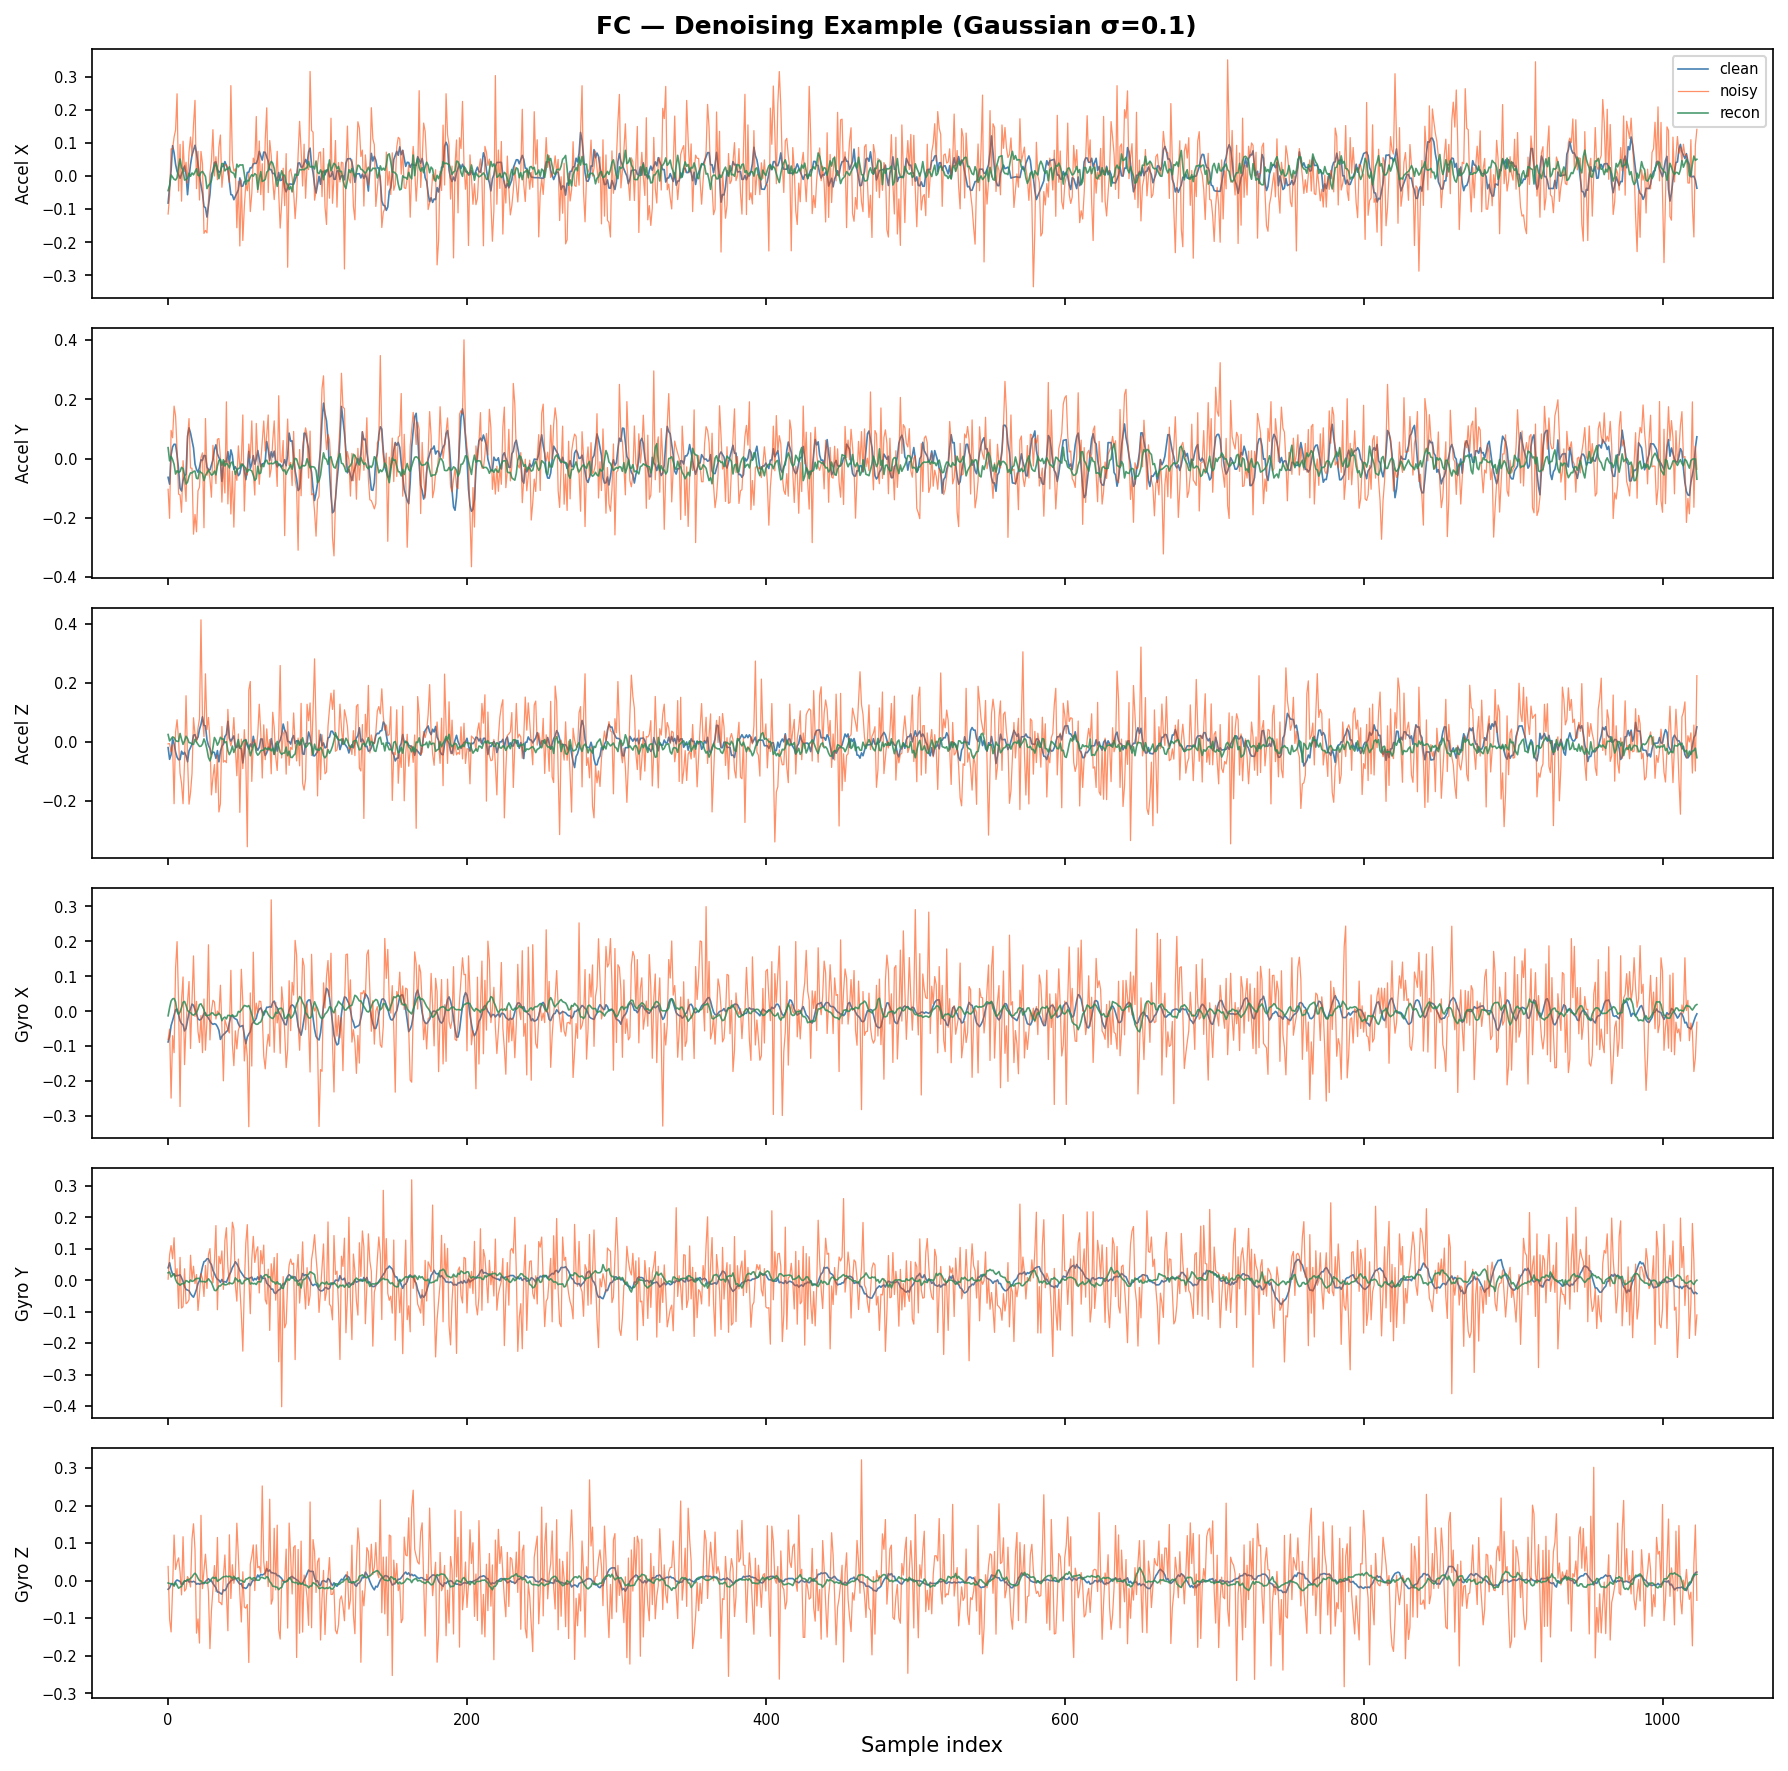
\includegraphics[width=0.48\linewidth]{../results/fc_reconstruction.png}
\end{center}
\caption{Signal reconstruction examples (6-channel wrist IMU, 1024 samples).
\figleft\ CNN autoencoder. \figright\ FC autoencoder.
Each panel shows three overlaid traces: clean (blue), noisy (red, $\sigma=0.1$
Gaussian), and reconstructed (green). Rows correspond to sensor channels
(Accel\,X/Y/Z, Gyro\,X/Y/Z).}
\label{fig:reconstructions}
\end{figure}

\subsection{Experiment 3: Latent Dimension Sweep}
\label{sec:exp-latent}

Each architecture is trained with bottleneck sizes
$d_z \in \{8, 16, 32, 64, 128, 256\}$, all other hyperparameters fixed.
Figure~\ref{fig:latent} plots test MSE and SNR$_\text{out}$ versus $d_z$.

\begin{figure}[h]
\begin{center}
\fbox{\rule[-.5cm]{0cm}{3cm} \rule[-.5cm]{8cm}{0cm}}
\end{center}
\caption{Latent dimension sweep: test MSE \figleft\ and SNR$_\text{out}$
\figright\ versus $d_z$ for all five architectures.
A U-shaped MSE curve is expected: very small $d_z$ underfits (insufficient
capacity), while very large $d_z$ may allow noise to pass through the bottleneck
unchanged.}
\label{fig:latent}
\end{figure}

We expect UNet-1D to be most robust at small $d_z$ since skip connections
bypass the bottleneck; the FC model should degrade fastest as it has no
structural regularisation beyond the bottleneck size.

\subsection{Experiment 4: Noise Robustness}
\label{sec:exp-noise}

Each architecture is trained with fixed Gaussian noise ($\sigma_\text{train} = 0.1$)
and evaluated at test-time levels $\sigma_\text{test} \in \{0.05, 0.1, 0.2, 0.4\}$.
Figure~\ref{fig:noise-robust} plots SNRi as a function of $\sigma_\text{test}$.

\begin{figure}[h]
\begin{center}
\fbox{\rule[-.5cm]{0cm}{3cm} \rule[-.5cm]{8cm}{0cm}}
\end{center}
\caption{Noise robustness: SNRi vs.\ test noise level $\sigma$.
Models are trained with $\sigma_\text{train}=0.1$.
A dashed horizontal line at SNRi\,$=0$ marks the no-improvement baseline.}
\label{fig:noise-robust}
\end{figure}

A counter-intuitive behaviour is expected and confirmed in preliminary runs: SNRi
\emph{increases} with $\sigma_\text{test}$.
At low $\sigma$ the noisy input is already close to clean, so the model's
residual reconstruction error dominates; at high $\sigma$ there is more noise
for the model to suppress, and the absolute SNR improvement grows.
This is a well-known property of fixed-threshold denoising estimators and is
\emph{not} a sign of incorrect evaluation.

\subsection{Experiment 5: Noise-Type Cross-Evaluation}
\label{sec:exp-noisetype}

Each architecture is trained independently on each of the four noise types, then
evaluated on all four types, producing a $4 \times 4$ SNRi matrix per
architecture.
The diagonal measures matched performance; off-diagonal entries quantify
out-of-distribution generalisation.
Figure~\ref{fig:noise-matrix} shows the resulting heatmaps.

\begin{figure}[h]
\begin{center}
\fbox{\rule[-.5cm]{0cm}{3.5cm} \rule[-.5cm]{8cm}{0cm}}
\end{center}
\caption{Noise-type cross-evaluation heatmaps (SNRi in dB).
Rows = training noise type; columns = test noise type.
Diagonal entries (bold) represent matched conditions;
off-diagonal entries reflect generalisation.
Green = positive SNRi (denoising gain); red = negative (noise amplification).}
\label{fig:noise-matrix}
\end{figure}

We hypothesise that Gaussian noise will generalise best across noise types due to
its smooth, isotropic corruption structure, while models trained on masking noise
will perform poorly on Gaussian (and vice versa), since the two regimes corrupt
qualitatively different aspects of the signal.

% ──────────────────────────────────────────────────────────────────
\section{Discussion}
\label{sec:discussion}

\textbf{Inductive bias matters.}
The five architectures span a spectrum from no temporal bias (FC) to strong
local bias (CNN, UNet), sequential bias (LSTM), and global attention
(Transformer).
Even with dropout regularisation, the FC model shows persistent train/val
overfitting because it must rediscover temporal locality from scratch, requiring
far more data than the 10\,K training windows available.
The CNN's local convolutions match the stationarity of IMU noise well.
The LSTM's final-hidden-state encoding (replacing mean pooling) was critical:
with mean pooling, training loss stagnated at $\approx$0.96 across all epochs
due to vanishing gradients over 1024 time steps.

\textbf{Skip connections for signal reconstruction.}
UNet-1D's skip connections create a direct path for preserving local signal
structure regardless of bottleneck capacity.
This is the architectural analogue of a residual connection
\citep{goodfellow2016deep}: the decoder need only learn the denoising
\emph{residual}, not reconstruct the signal from scratch.
The substantially lower MSE of UNet-1D (observed from epoch~1 in preliminary
runs) strongly supports this interpretation.

\textbf{Hybrid loss and tremor preservation.}
The spectral $L_1$ term in Eq.~\eqref{eq:loss} encourages the model to match the
magnitude spectrum of the reconstruction to that of the clean signal.
Without this term, a purely MSE-minimising model can achieve low reconstruction
error by smoothing transients, which suppresses the 4--6\,Hz tremor content.
The TremorMAE metric operationalises this concern: a model with low MSE but high
TremorMAE is clinically harmful even if statistically ``good.''

\textbf{Metric consistency.}
Training uses the hybrid loss (MSE + $\alpha \cdot$ spectral $L_1$), while
cross-architecture evaluation uses pure MSE and SNRi.
These are on different scales and should never be compared directly; only test
MSE values are used for ranking.
The hybrid loss is a \emph{training objective}, not an evaluation criterion.

% ──────────────────────────────────────────────────────────────────
\section{Conclusion}
\label{sec:conclusion}

We presented a comprehensive denoising autoencoder study for Parkinson's Disease
wrist IMU signals, implementing five architectures across four noise regimes on
the PADS dataset.
Key design choices—subject-level splitting, per-channel z-score normalisation,
hybrid spectral loss, and overlapping-window augmentation—address practical
challenges specific to biomedical wearable data.

The study demonstrates that architectural inductive bias is the dominant factor
in denoising performance at this dataset scale:
skip connections (UNet-1D) and global attention (Transformer) substantially
outperform architectures that process signals through a strict information
bottleneck without structural priors.
The frequency-domain loss term provides additional regularisation that
encourages spectral fidelity beyond MSE, which is clinically meaningful given
the diagnostic importance of the 4--6\,Hz tremor band in Parkinson's Disease.

\subsubsection*{Author Contributions}
Wanghley Soares Martins led the dataset integration, model implementation
(UNet-1D, Transformer, multi-channel refactoring), training pipeline
(hybrid loss, subject-level splitting, data augmentation), experiment
infrastructure (timestamped run directories, noise-type cross-evaluation), and
result analysis.
Yibei Gou contributed the baseline architectures (FC, CNN, LSTM), evaluation
metrics (MSE, SNR, SNRi), hyperparameter grid search, noise robustness
experiment, and the initial training loop.

\bibliography{iclr2024_conference}
\bibliographystyle{iclr2024_conference}

% ──────────────────────────────────────────────────────────────────
\appendix
\section{Implementation Details}
\label{app:impl}

\subsection{Codebase Structure}

\begin{center}
\begin{tabular}{ll}
\toprule
\textbf{File} & \textbf{Role} \\
\midrule
\texttt{pads\_dataset.py} & Dataset loader, subject split, z-score normalisation \\
\texttt{models.py}        & FC, CNN, LSTM, UNet-1D, Transformer architectures \\
\texttt{noise.py}         & Gaussian, masking, impulse, sinusoidal noise functions \\
\texttt{train.py}         & Training loop, hybrid loss, validation, checkpointing \\
\texttt{metrics.py}       & MSE, SNR, SNRi, tremor-band power MAE \\
\texttt{experiments.py}   & Five experiment runners + JSON/PNG output \\
\texttt{visualize.py}     & Signal plots, training curves, heatmaps \\
\texttt{config.py}        & Hyperparameters, dataset paths, sweep ranges \\
\texttt{main.py}          & CLI entry: \texttt{--exp \{all|arch|latent|noise|noise\_types|hyperparam\}} \\
\bottomrule
\end{tabular}
\end{center}

\subsection{Reproducibility}

All experiments use a fixed random seed (42) for subject splitting and model
initialisation.
The full pipeline can be reproduced with:

\begin{verbatim}
python main.py --exp all --epochs 100
\end{verbatim}

Results are written to \texttt{results/YYYYMMDD\_HHMMSS/} including a
\texttt{run\_config.json} snapshot of all settings.

\end{document}
